\documentclass[12pt, a4paper]{article}

% Packages and Formatting
\usepackage{../../sub/mystyle_general}
\usepackage{../../sub/mystyle_article}


\title{Lista 3 - Introdução a Análise de Dados \\
	Funções}
\author{Guilherme Masuko}
\date{April 2023}
%\affil{}


\begin{document}
	
% Title Page
\clearpage
\maketitle
\thispagestyle{empty}

\textbf{Curso de Cálculo:} \href{https://cursos.takhe.com.br/}{Takhe}

\textbf{Professor:} Douglas Bokliang

\vspace{1cm}



\textbf{Questão 1}

A convexidade de uma função é dada pela segunda derivada (isso sob a condição de continuidade da função). A definição formal de convexidade de função pode ser encontrada clicando \href{https://pt.wikipedia.org/wiki/Fun\%C3\%A7\%C3\%A3o\_convexa}{aqui} (pode assustar, mas não se preocupe, utilizaremos um teorema para resolver o exercício).

\begin{quote}
	Teorema\footnote{\url{https://www.professores.uff.br/hjbortol/wp-content/uploads/sites/121/2017/09/gma00108-parte-21.pdf}}:
	
	Seja $I$ um intervalo contido no domínio de uma função $f$. Suponha que $f$, $f^{\prime}$ e $f^{\prime \prime}$ sejam contínuas em $I$. 
	
	\begin{itemize}
		\item Se $f^{\prime \prime} (x) > 0$ para todo $x \in I$, então $f$ é uma função convexa no intervalo $I$.
		
		\begin{figure}[h]
			\caption{Função Convexa}
			\centering
			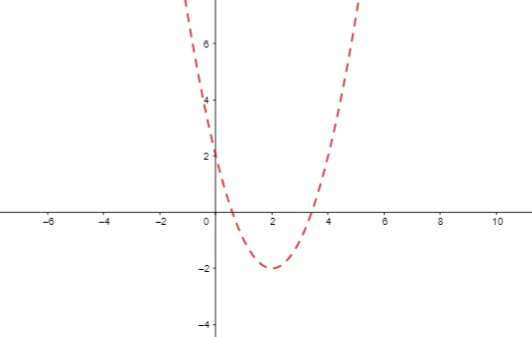
\includegraphics[scale=.73]{images/convexa.jpg}
			\label{fig:convexa}
		\end{figure}
	
	
		\item Se $f^{\prime \prime} (x) < 0$ para todo $x \in I$, então $f$ é uma função côncava no intervalo $I$.
		
		\begin{figure}[h]
			\caption{Função Côncava}
			\centering
			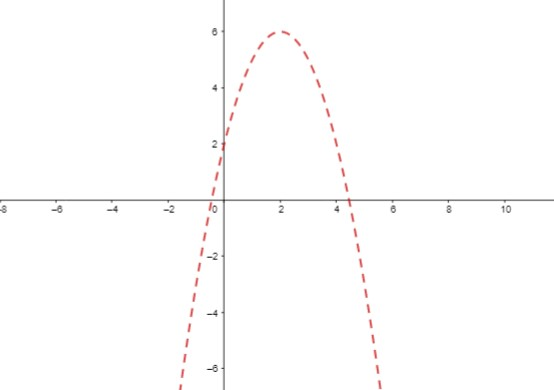
\includegraphics[scale=.73]{images/concava.jpg}
			\label{fig:concava}
		\end{figure}
	\end{itemize}
\end{quote}

Isso quer dizer que para funções do segundo grau contínuas, o coeficiente $a$ determina a convexidade da função. Seja $f(x) = ax^2 + bx + c$.

\begin{align*}
	f^{\prime} (x) &= 2ax + b \\
	f^{\prime \prime} (x) &= 2a
\end{align*}

Ou seja, se $a > 0$, então a função $f$ é convexa e se $a < 0$, então a função é côncava.

Crie uma função que receba os três coeficientes de uma função do segundo grau como parâmetros e retorne a convexidade da função (\texttt{'convexa'} ou \texttt{'côncava'}).

Teste sua função para as seguintes equações:

\begin{itemize}
	\item $f(x) = -2x^2 + 4x + 6$
	\item $f(x) = x^2 - 4x + 10$
\end{itemize}



\textbf{Questão 2}

Um ponto crítico\footnote{\url{https://pt.wikipedia.org/wiki/Ponto\_cr\%C3\%ADtico\_(fun\%C3\%A7\%C3\%B5es)}}
 de uma função é um ponto no domínio de uma função onde a primeira derivada não existe ou é nula. Os pontos críticos serão sempre pontos de máximos ou mínimos locais ou pontos de inflexão.
No caso de funções do segundo grau, $f(x) = ax^2 + bx + c$, o ponto crítico da função é encontrado da seguinte maneira.

\begin{align*}
	f^{\prime} (x^{\star}) &= 2ax^{\star} + b = 0\\
		x^{\star} &= -\frac{b}{2a}
\end{align*}


Crie uma função que receba os três coeficientes de uma função do segundo grau como parâmetros e retorne o ponto crítico e o valor da função avaliado no ponto crítico, respectivamente, $x^{\star}$ e $f (x^{\star})$.

Teste sua função para as seguintes equações:

\begin{itemize}
	\item $f(x) = -2x^2 + 4x + 6$
	\item $f(x) = x^2 - 4x + 10$
\end{itemize}



\textbf{Questão 3}

Utilizando as funções criadas nas questões 1 e 2, crie uma função que receba os coeficientes de uma função do segundo grau como parâmetros e retorne o ponto crítico e se ele é um ponto de máximo ou mínimo. 

Dica: Se uma função é estritamente côncava em um intervalo $I$, um ponto crítico nesse mesmo intervalo é um ponto de máximo local. Se uma função é estritamente convexa em um intervalo $I$, um ponto crítico nesse mesmo intervalo é um ponto de mínimo local.

Teste sua função para as seguintes equações:

\begin{itemize}
	\item $f(x) = -2x^2 + 4x + 6$
	\item $f(x) = x^2 - 4x + 10$
\end{itemize}



\textbf{Questão 4}

É possível esboçar o gráfico de uma função quando se sabe características importantes dela, por exemplo, suas raízes, sua convexidade, seu ponto crítico e o valor da função neste ponto. Crie uma função que receba os coeficientes de uma função do segundo grau como parâmetros e retorne suas raízes (use a função feita na Lista 1), seu ponto de máximo ou mínimo e o valor da função neste ponto (use a função feita na questão anterior).

Teste sua função para as seguintes equações:

\begin{itemize}
	\item $f(x) = -2x^2 + 4x + 6$
	\item $f(x) = x^2 - 4x + 10$
\end{itemize}


	
\end{document}